\documentclass[a4paper,11pt]{article}
\usepackage{amscd}
\usepackage{amsmath}
\usepackage{amssymb}
\usepackage{amsthm}
\usepackage{fontenc}
\usepackage{latexsym}
\usepackage[english]{babel}
\usepackage[utf8]{inputenc}
\usepackage[T1]{fontenc}
\usepackage[a4paper]{geometry}
\usepackage{tikz-cd}
\usepackage{tikz}
\usepackage{mathrsfs}
\usepackage{cancel}
\usepackage{blindtext}

\newtheorem{theorem}{Theorem}[section]
\newtheorem{proposition}[theorem]{Proposition}
\newtheorem{lemma}[theorem]{Lemma}
\newtheorem{corollary}[theorem]{Corollary}


\theoremstyle{remark}
\newtheorem{example}[theorem]{\textbf{Example}}
\newtheorem{observation}[theorem]{\textbf{Observation}}
\newtheorem{Remark}[theorem]{\textbf{Remark}}

\theoremstyle{definition}
\newtheorem{definition}[theorem]{Definition}


\newcommand{\N}{\mathbb{N}}
\newcommand{\Z}{\mathbb{Z}}
\newcommand{\R}{\mathbb{R}} 


%stili per tikz%
\tikzstyle{place}=[circle,draw=black!100,fill=black!100,thick,
inner sep=0pt,minimum size=2mm]
\tikzstyle{shuffle}=[circle,draw=black!100,fill=black!100,thick,
inner sep=0pt,minimum size=0.01mm]

\begin{document}


\title{On the multisimplicial cup product}
\date{}
\author{Andrea Pizzi and Paolo Salvatore  \footnote{The third author acknowledges support from 
the MIUR Excellence Department Project MATH@TOV CUP E83C18000100006}
 }

	
\maketitle


\abstract{We define a cup product on the cochain complex of a multisimplicial set, that is compatible with the classical cup product on the cochain complex of the diagonal simplicial set via the Eilenberg-Zilber map. This helps to speed up cochain level computations for multisimplicial complexes. 
}

	
\section{Introduction}

The cochain complex $C^*(K)$ of a simplicial set $K$ is equipped with the classical Alexander-Whitney cup product that makes into a
differential graded algebra.
Our primary goal is to extend this product to the case of multisimplicial sets.  Let us consider a $k$-fold simplicial set $X$, that is a contravariant functor from $(\Delta)^k$ to the category of sets. The restriction to the diagonal  $\Delta \subset (\Delta)^k$ defines a simplicial set $X^D$. There is a notion 
of geometric realization $|X|$ of a $k$-fold simplicial set $X$, that is a CW complex with a cell $e_x$ for each non-degenerate multisimplex $x$, with a characteristic map from a product of simplexes  $$\Delta_{i_1} \times \dots \times \Delta_{i_k} \to e_x$$ This extends the classical case where the characteristic map has a single simplex as domain. 
Quillen proved in 
\cite{Quillen} that there is  a natural homeomorphism of realizations $|X| \cong |X^D|$. Under this homeomorphism the cells of $|X^D|$ arise from those
of $|X|$ by subdividing $k$-fold products of simplexes into simplexes. This procedure is described combinatorially by the Eilenberg-Zilber quasi-isomorphism $$EZ:C_*(X) \to C_*(X^D)$$ that induces a quasi-isomorphism on normalized chains 
%meglio N invece di C_N
$N_*(X) \to N_*(X^D)$ after quotienting out degenerate chains.
 As in the classical simplicial case, the projection $C_*(X) \to N_*(X)$ onto normalized chains 
is a quasi-isomorphism.

\medskip

 We prove in Theorem \ref{algebra}  %quale?
 that the cochain complex $C^*(X)$ is equipped with a differential graded algebra structure.
 The product is the natural extension to the multisimplicial case of the cup product  defined by the Alexander-Whitney formula, by
  evaluating cochains on front and rear faces in all multisimplicial directions. %formula?
  We prove in section \ref{ultima}
   that the dual Eilenberg-Zilber map
 $$EZ^*:C^*(X^D) \to C^*(X)$$ %provato dove?
  is a quasi-isomorphism of differential graded algebras, where the source is equipped with the classical cup product.  
 Furthermore the Eilenberg-Zilber map restricts to a quasi-isomorphism $$N^*(X^D) \to N^*(X)$$ of sub-algebras of normalized cochains.   
 Our result is very useful for computations, since multisimplicial models of spaces have a signficantly smaller number of non-degenerate cells then their simplicial models.
So $N^*(X)$ is much smaller than $N^*(X^D)$, but it contains the same information up to homotopy, 
allowing for example 
to calculate Massey products, and to detect its formality. 
As an example we consider a family of multisimplicial sets $Sur(k)$ defined  by McClure and Smith, see \cite{MS},  modelling euclidean configuration spaces.
%the surjection operad chain complex $\chi(k)$ he normalized chain complex of a $k$-fold simplicial set for any $k$. %The sub-operad $\Chi_2$ is also known as cactus operad.
The proof by the second author of the non-formality of the cochain algebra of planar configuration spaces in \cite{formality}  used the Barratt-Eccles simplicial model and the classical cup product.
Our new product on the multisimplicial McClure-Smith models makes the computation much simpler and faster, paving the way for an extension to higher dimensions. 
%per esempio dire i numeri..

\medskip

%In Theorem \ref{} we extend the d.g. algebra structure on $C^{*N}(X)$  above to an $E_\infty$ algebra structure, so that 
%$EZ: C^{*N}(X^D) \to C^{*N}(X)$ is a quasi-isomorphism of $E_\infty$-algebras. The $E_\infty$-operad acting here is exactly $\chi$, and its action 
%on the source is that defined by McClure and Smith \cite{MS}. 

%Composing with the standard quasi-isomorphism  
%$S^{*N}( |X^D| ) \cong C^{*N}(X^D)$ from normalized singular cochains on $|X^D| \cong |X|$, we are able to recover from the combinatorics of $C^{*N}(X)$   

The results of this paper appeared first in the B.Sc. thesis of the first author, University of Rome Tor Vergata (2019), written under the guidance of the second author.
%ringraziamenti al progetto solito

\section{Normalized complexes of multisimplicial modules}
%troppi normalizzati
We always consider modules over a commutative ring $R$ that will be usually be dropped from the notation. 

\begin{definition}	
Let $X$ be a simplicial module, i.e. a contravariant functor from $\Delta$ to the category of $R$-modules.
The chain complex associated to $X$ is $C_{*}(X)=X_*$
%	\begin{equation*}
%	\dots \rightarrow X_{n+1} \rightarrow X_{n} \rightarrow X_{n-1} \rightarrow \dots
%	\end{equation*}
with differential $\partial_{n}:C_{n}(X) \rightarrow C_{n-1}(X)$ given by the formula 
	\begin{equation*}
	\partial_{n}= \sum_{i=0}^{n} (-1)^{i} d_{i}
	\end{equation*}
where each $d_{i}:X_n \to X_{n-1}$ is a  face map, the image of $\delta_{i}:[n-1] \to [n]$ via $X$.
\end{definition}

\begin{definition}
A multisimplicial (or $k$-fold simplicial) module (resp. set) $X$ is a functor from $(\Delta)^{k}$ to the category of $R$-modules (resp. sets), for some positive integer $k$. An element $x \in X_{i_1,\dots,i_k}$ is called a $(i_1,\dots,i_k)$-multisimplex. 
The face map 
$$d_i^j:X_{i_1,\dots,i_j,\dots,i_k} \to X_{i_1,\dots,i_j-1,\dots,i_k}$$ in direction $j$ for $1 \leq j \leq k$
and $0 \leq i_j \leq j$, is the image via $X$ of $(id,\dots,id, \delta_{i_j},id, \dots,id)$. The degeneracy map $$s^l_i:X_{j_1,\dots,j_l, \dots,j_k} \to X_{j_1,\dots,j_l+1,\dots,j_k}$$ in direction $l$ is the image via $X$ of $(id, \dots,id,\sigma_i,id,\dots,id)$.
\end{definition}
 Clearly faces and/or degeneracies in different directions commute with each other.



\begin{definition}
%naturali
The associated chain complex $C_{*}(X)$ of a multisimplicial module is defined by
	\begin{equation*}
	C_{n}(X)= \bigoplus_{i_{1}+\dots +i_{k}=n}X_{i_{1},\dots,i_{k}}
	\end{equation*}
%On $X$ we have a chain complex (simplicial) in each direction $i_{j}$, with $0\le j \le k$, with differential
If we define
	\begin{equation*}
	\partial_{i_{j}}=\sum_{t=0}^{i_{j}} (-1)^{t+i_{1}+\dots+i_{j-1}}d^j_{t}: X_{i_{1},\dots,i_{j},\dots,i_{k}}\rightarrow X_{i_{1},\dots,i_{j}-1,\dots,i_{k}}
	\end{equation*}
then the multisimplicial differential on $C_{*}(X)$ is defined 
on the summand $X_{i_{1},\dots,i_{j},\dots,i_{k}}$
by the formula 
	\begin{equation*}
	\label{differenziale}
	\partial = \partial_{i_{1}}+\dots+\partial_{i_{k}}
	\end{equation*}
\end{definition}


As usual the cochain complex $C^*(X)$ of a (multi)simplicial module $X$ is the linear dual of $C_*(X)$.  
A standard example of multisimplicial $R$-module is $X=RK$, with $K$ multisimplicial set, and $X_{i_1,\dots,i_k}$ the free $R$-module
on $K_{i_1,\dots,i_k}$.

%Recall that a degeneracy $s_i:X_n \to X_{n+1}$ of a simplicial module, for $0 \leq i \leq n$ is the image via $X$ of $\sigma_i:[n+1] \to [n]$.
The following definition extends the standard definition of the simplicial case.
%\newpage
%\section{Technical Results}
\begin{definition}
A multisimplex of a multisimplicial module (or multisimplicial set)  is said to be {\em degenerate} if it is in the image of a degeneracy.
\end{definition}

%We need some technical results about multisimplicial chain complexes to deal with \textit{normalized multisimplicial chain complexes}. First of all we recall the following theorem:




We define next the normalized chain complex of a multisimplicial module.

\begin{definition}
Let $X$ a multisimplicial module. We define $D_{*}(X)$ to be the subcomplex of $C_{*}(X)$ generated by all degenerate elements, in each dimension $n$, i.e. $D_{0}(X)=0$ and:
	\begin{equation*}
	\resizebox{0.5\hsize}{!}{$%
	\begin{split}
    D_{n}(X)= 
    \sum_{\begin{split}
    	& 0 \leq i_l \leq j_l \\
    	j_{1}+&\dots +j_{k}=n-1 \\
    	\end{split}} 
    s_{i_l}^{l}X_{j_{1},\dots,j_{k}} \\
	\end{split}
    $%
    }%
	\end{equation*}
%where the set $S_{n-1}(X)$ is the following:
%	 $$\left\lbrace 
%	 \begin{split}
%	 &s_{i}^{j_{l}} \text{ is a degeneracy in }  X_{j_{0},\dots,j_{k}} \text{ with } j_{0}+\dots+j_{k}=n-1 \text{ and } 0\geq i \geq j_{l} \\ &\text{so that } s_{i}^{j_{l}}X_{j_{0},\dots,j_{k}}=X_{j_{0},\dots,j_{l}+1,\dots,j_{k}} \subset C_{n}(X) \\
%	 \end{split}	 
%	 \right\rbrace$$ 
By the multisimplicial identities $D_{*}(X)$ is closed under the differential $\partial$, so it is actually a subcomplex of $C_*(X)$.
 The quotient $C_{*}(X)/ D_{*}(X) = N_*(X)$  is called the \textit{normalized chain complex of $X$}.
\end{definition}

A classical result is the following normalization theorem.
\begin{theorem}(Normalization Theorem 6.1, Chap. 8 in  \cite{maclanehomology})
	\label{normalizationtheorem}
For each simplicial module X the canonical projection $\pi:C_{*}(X)\rightarrow N_*(X)$ is a chain equivalence.
\end{theorem}

The result extends to multisimplicial modules.  

%Indeed, that is, at index n, the same module with degeneracy elements coming from $C_{n-1}(X)$ omitted.

\begin{theorem}(Generalized Normalization Theorem)
   \label{generalizednormalizationtheorem}
For each multisimplicial module X the canonical projection $\pi:C_{*}(X)\rightarrow N_*(X)$ is a chain equivalence.:
\end{theorem}
\begin{proof}
%rifare
The proof is a slight variation of the proof in \ref{normalizationtheorem}.
Consider the degree one map 
$t_j^l:C_*(X) \to C_{*+1}(X)$   given by $t_j^l(x)=(-1)^{j+i_1+\dots+i_{l-1}} s_j^l(x)$
for a multisimplex $x \in X_{i_1,\dots,i_k}, \; 1 \leq l \leq k$ and $0 \leq j \leq i_l$.
Then $$h_j^l = 1-\partial t_j^l - t_j^l \partial :C_*(X) \to C_*(X)$$ is a chain map,
and $t_j^l$ a homotopy between $h_j^l$ and the identity. We set $h^l =h^l_0 \circ h^l_1 \circ \dots $ for $l=1,\dots,k$. Then we set 
$h= h^1 \circ \dots \circ h^k$. Notice that the chain maps $h^1,\dots,h^k$ commute with each other. We conclude following the proof by Mac Lane.  %controllare
\end{proof}


%\begin{observation}
%	In the proof of Theorem \ref{generalizednormalizationtheorem} is important to outline that $\pi_{j}$ is defined only after chosing the string $(i_{0},\dots,i_{k})$, and which indices are fixed. This observation is helpful to keep in mind to eventually find the homotopy explicitly.
%\end{observation}

%Consider initially the modules $X_{1}$, $X_{2}\times \dots \times X_{k}\, $. By Theorem \ref{EZtheorem} we have the chain equivalence
%	$$C_{*}^{N}(X_{1}\otimes X_{2}\otimes \dots \otimes X_{k})\leftrightarrow C_{*}^{N}(X_{1})\otimes  C_{*}^{N}(X_{2}\times \dots \times X_{k})$$
%At step $i$ consider the modules $X_{i}$, $X_{i+1}\otimes \dots \otimes X_{k}$. Inductively we obtain the wanted result.
%\end{proof}


\




\section{Eilenberg-Zilber maps}





We recall first the classical Eilenberg-Zilber map, and then define its multisimplicial version.
Let us recall the definition of shuffle.

\begin{definition}
Let $a_{1},\dots,a_{k}\in\mathbb{N}$. 
%and $k+1$ words $w_{0}=\varepsilon_{1}\dots \varepsilon_{a_{0}}$, \dots, $w_{k}=\varepsilon_{1}\dots \varepsilon_{a_{k}}$ we obtain a $(a_{0},\dots,a_{k})$-\textit{shuffle} concatenating $w_{0}, \dots,w_{k}$,
%	$$c_{1}\dots c_{a_{0}+\dots+a_{k}}=w=w_{0}, \dots,w_{k}$$
%and commuting indices $\left\lbrace 1,2,\dots,a_{0}+\dots+a_{k}\right\rbrace $ 
A permutation $\sigma\in S_{a_{1}+\dots+a_{k}}$ such that  $\sigma(1)<\dots<\sigma(a_{1})\, ,  \, \sigma(a_{1}+1)<\dots<\sigma(a_{1}+a_{2})\; \dots\; \sigma(a_{1}+\dots+a_{k-1}+1)<\dots<\sigma(a_{1}+\dots+a_{k})$  
%\omega=c_{\sigma(1)}\dots c_{\sigma(a_{0}+\dots+a_{k})}
is called an $(a_{1},\dots,a_{k})$-\textit{shuffle}.
% In our case we use numbers' words $\left[ n\right] = \left\lbrace 0,1,2,\dots,n\right\rbrace $.
\end{definition}



Equivalently an $(a_1,\dots,a_k)$-shuffle corresponds to a collection of monotone maps
$$\pi_i:[a_1+\dots+a_k] \to [a_i]$$ for $i=1,\dots,k$  such that for each $j=0,\dots,a_1+\dots+a_k-1$ there is exactly 
one index $l \in \{1 \dots k\}$ satisfying $\pi_l(j+1)=\pi_l(j)+1$, and $\pi_i(j+1)=\pi_i(j)$ for all $i \neq l$.
Geometrically this collection $(\pi_1,\dots,\pi_k)$ represents a sequence of $(a_1+\dots+a_k)$  moves in a lattice of integral points with $(k+1)$-coordinates, starting at the origin, and moving in a single direction at each stage, until the point $(a_1,\dots,a_k)$ is reached. 
The associated permutation sends $j+1$ to $a_1+\dots+a_{l-1}+\pi_l(j+1)$. 
We denote the set of $(a_1,\dots,a_k)$-shuffles by $\mathfrak{sh}(a_{1},\dots,a_{k})$.

\begin{example}
	\label{esempioshuffle}
%Let $a=\left[0,1,2,3,4\right]=\left[ 4\right] $ and $b=\left[0,1,2\right] = \left[ 2\right]$. To simplify the notation we modify numbers of the second string like: $b=\left[0,5,6\right] $.
The permutation  $\pi=(1, 2, 5, 3, 4, 6) $ is a $\left( 4,2\right)$-shuffle.
 Indeed we have that  $\pi(1)=1 < \pi(2)=2 < \pi(3)=4 < \pi(4)=5 $ and  $\pi(5)=3 < \pi(6)=6 $.
 The corresponding monotone maps are
 $\pi_1:[0,6] \to [0,4]$ such that 
 $\pi_1(0)=0, \pi_1(1)=1,  \pi_1(2)=2=\pi_1(3), \pi_1(4)=3, \pi_1(5)=4=\pi_1(6)$ and
 $\pi_2:[0,6] \to [0,2]$ such that $\pi_2(0)=0=\pi_2(1)=\pi_2(2), \pi_2(3)=1=\pi_2(4)=\pi_2(5), \pi_2(6)=2$.
 The corresponding path is indicated in red in the figure.
\end{example}


%In the definition i mention some \textit{'grids'}. Indeed we can figured them out as in the following grid:


\begin{figure}[tbh] %simplesso singolare%
	\label{figura4.1}
	\centering
	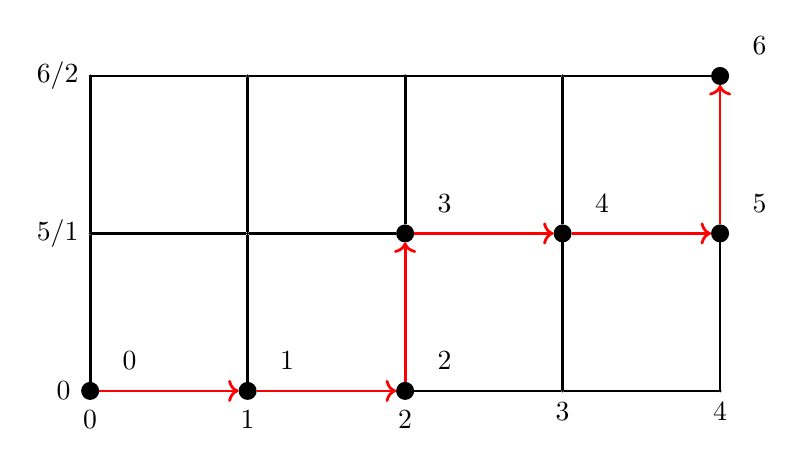
\begin{tikzpicture}[scale=2,line width=1pt]
	
	\node  (v0)   at (0,0) [place,label=below:$0$,label=left:$0$] {};
	\node  (v1)   at (1,0) [place,label=below:$1$] {};
	\node  (v2)   at (2,0) [place,label=below:$2$] {};
	\node  (v3)   at (3,0) [shuffle,label=below:$3$] {};
	\node  (v4)   at (4,0) [shuffle,label=below:$4$] {};
	\node  (v5)   at (0,1) [shuffle,label=left:$5/1$] {};
	\node  (v6)   at (1,1) [shuffle] {};
	\node  (v7)   at (2,1) [place] {};
	\node  (v8)   at (3,1) [place] {};
	\node  (v9)   at (4,1) [place] {};
	\node  (v10)   at (0,2) [shuffle,label=left:$6/2$] {};
	\node  (v11)   at (1,2) [shuffle] {};
	\node  (v12)   at (2,2) [shuffle] {};
	\node  (v13)   at (3,2) [shuffle] {};
	\node  (v14)   at (4,2) [place] {};
	\node  (v15)   at (0.25,0) [label=above:$0$] {};
	\node  (v16)   at (1.25,0) [label=above:$1$] {};
	\node  (v17)   at (2.25,0) [label=above:$2$] {};
	\node  (v18)   at (2.25,1) [label=above:$3$] {};
	\node  (v19)   at (3.25,1) [label=above:$4$] {};
	\node  (v20)   at (4.25,1) [label=above:$5$] {};
	\node  (v21)   at (4.25,2) [label=above:$6$] {};
	
	\draw [->,draw=red!100] (v0) to (v1);
	\draw [->,draw=red!100] (v1) to (v2);
	\draw [-] (v2) to (v3);
	\draw [-] (v3) to (v4);
	\draw [-] (v5) to (v6);
	\draw [-] (v6) to (v7);
	\draw [->,draw=red!100] (v7) to (v8);
	\draw [->,draw=red!100] (v8) to (v9);
	\draw [-] (v10) to (v11);
	\draw [-] (v11) to (v12);
	\draw [-] (v12) to (v13);
	\draw [-] (v13) to (v14);
	\draw [-] (v0) to (v5);
	\draw [-] (v5) to (v10);
	\draw [-] (v1) to (v6);
	\draw [-] (v6) to (v11);
	\draw [->,draw=red!100] (v2) to (v7);
	\draw [-] (v7) to (v12);
	\draw [-] (v3) to (v8);
	\draw [-] (v8) to (v13);
	\draw [-] (v4) to (v9);
	\draw [->,draw=red!100] (v9) to (v14);
		
	\end{tikzpicture}
	\caption{$\left( 4,2\right)$-shuffle of example \ref{esempioshuffle}. }
\end{figure}



%put here classical 
\begin{definition}
For simplicial modules $X$ and $Y$
the classical Eilenberg-Zilber map 
$$EZ:N_*(X) \otimes N_*(Y) \to N_*(X \otimes Y)$$
is defined by  $$EZ(x \otimes y) = \sum_{\pi \in \mathfrak{sh}(p,q)} sgn(\pi)  X(\pi_1)(x) \otimes X(\pi_2)(y)$$
for $x \in X_p$ and $y \in Y_q$. 
\end{definition}


\begin{theorem}(Classic Eilenberg-Zilber Theorem)
	\label{EZtheorem}
For simplicial modules $X$ and $Y$ 
	$$EZ:  N_*(X)\otimes N_*(Y)  \to N_*(X\otimes  Y)$$ is a well defined and natural chain equivalence
\end{theorem} 

A natural inverse equivalence to the Eilenberg-Zilber map is the Alexander-Whitney map. 


%only normalized

\begin{definition}
For simplicial modules $X_1,\dots,X_k$ the multivariable Eilenberg-Zilber chain map
$EZ: N_{*}(X_{1})\otimes\dots \otimes N_{*}(X_{k}) \to N_*(X_1 \otimes \dots \otimes X_k)$ 
is defined by  $$EZ(x_1 \otimes \dots \otimes x_k) =  \sum_{\pi \in \mathfrak{sh}(a_{1},\dots,a_{k})} sgn(\pi) X_1(\pi_{1})(x_1) 
\otimes  \dots \otimes  X_k(\pi_k)(x_k)$$
\end{definition}
It is easy to verify that this chain map can also be obtained by iterating the classical map. %verifica?
%In particular $EZ$ induces a map on normalized cochains.
By applying repeatedly theorem  \ref{EZtheorem}% and using the normalization theorem \ref{normalizationtheorem}
 we obtain the following corollary.

\begin{corollary}(Extension of Eilenberg-Zilber Theorem)
\label{extez}
For simplicial modules $X_{1},\dots,X_{k}$  
%	$$EZ:  C_{*}(X_{1})\otimes\dots \otimes C_{*}(X_{k}) \to C_{*}(X_{1}\otimes \dots \otimes X_{k})$$ 
%is a natural chain equivalence, and so is the induced chain map
	$$EZ: N_*(X_{1})\otimes\dots \otimes N_*(X_{k}) \to N_*(X_{1}\otimes \dots \otimes X_{k})$$
is a natural chain equivalence.	
\end{corollary}
%\begin{proof}
A natural inverse equivalence is the iterated Alexander-Whitney map.

For the multisimplicial version we need the following definition.
\begin{definition}
Given a multisimplicial module (or set ) $X:\Delta^k \to {\bf Set}$ its {\em diagonal}  $X^D:\Delta \to {\bf Set}$ 
is the simplicial module (or set) that is the restriction of $X$ to the diagonal copy $\Delta \subset \Delta^k$.
\end{definition}

Observe now that if $X$ is a multisimplicial module, $\pi$ an $(a_1,\dots,a_k)$-shuffle, and $x \in X_{a_1,\dots,a_k}$ a multisimplex, then 
$$X(\pi_{1}, \dots, \pi_k) (x) \in X^D_{a_1+ \dots + a_k}$$ is in the diagonal.
We can now define the multisimplicial Eilenberg-Zilber map.


\begin{definition}%(Multisimplicial Eilenberg-Zilber map)
Let $X$ be a multisimplicial module.
The multisimplicial \textit{Eilenberg-Zilber map}, $\mathit{EZ}:N_*(X)\rightarrow N_*(X^{D})$, is defined as follows:
For a given $(a_{1},\dots,a_{k})$-multisimplex $x$



	\begin{equation*}
	\label{EZ}
	\mathit{EZ}(x) = 	\sum_{\pi \in \mathfrak{sh}(a_{1},\dots,a_{k})} {sgn(\pi)} X(\pi_{1}, \dots, \pi_k) (x)   
	\end{equation*}
%where i define $\bar{\pi}$ as $\bar{\pi}(i)=\pi(i)-1$ for each $1\le i \le a_{0}+\dots +a_{k}$.
	
%Symbols used in the formula are abbreviations to make the notation simpler and represent the following expressions:
%	\begin{equation*}
%	\begin{split}
%	& (s^{a_{i}}_{i\ne0} )_{\bar\pi{(1)}}^{\bar\pi{(a_{0})}} = \left[  s_{\bar{\pi}(1)}^{a_{i} }\dots s_{\bar{\pi}(a_{0})}^{a_{i}}\right] _{i\ne0} \qquad \text{(for each } i\ne0)\\
%	& (s^{a_{i}}_{i\ne1})_{\bar\pi{(a_{0}+1)}}^{\bar\pi{(a_{0}+a_{1})}} = \left[ s_{\bar{\pi}(a_{0}+1)}^{a_{i} }\dots s_{\bar{\pi}(a_{0}+a_{1})}^{a_{i}}\right]_{i\ne1}  \qquad \text{(for each } i\ne1)\\
%	& \dots \\
%	& (s^{a_{i}}_{i\ne k})_{\bar\pi{(a_{0}+a_{1}+1)}}^{\bar\pi{(a_{0}+\dots+a_{k})}} = \left[ s_{\bar{\pi}(a_{0}+\dots +a_{k-1}+1)}^{a_{i} }\dots s_{\bar{\pi}(a_{0}+\dots +a_{k})}^{a_{i}}\right]_{i\ne k}  \qquad \text{(for each } i\ne k)
%	\end{split}
%	\end{equation
\end{definition}
We can extend Theorem 2.5, chap. 4 in \cite{GJ}, that is about bisimplicial modules, to the general multisimplicial case as follows:
\begin{theorem}
	\label{generalGJtheorem}
Let $X$ be a multisimplicial module.  Then $EZ: N_*(X) \to N_*(X^D)$ 
is a natural chain equivalence.
\end{theorem}
\begin{proof}
The proof is similar to that of Theorem 2.5, chap.4 in \cite{GJ} adapted to multisimplicial modules, using corollary \ref{extez}.
Consider 
the standard multisimplicial set $$\Delta_{i_1,\dots,i_k} := Hom(\_,([i_1],\dots,[i_k]))$$
Corollary \ref{extez} proves the theorem
for the standard multisimplicial module $X= R  \Delta_{i_1,\dots,i_k}$.
Namely the simplicial set  $\Delta_{i_1} \times \dots \times \Delta_{i_k}$ is isomorphic to the diagonal $\Delta_{i_1,\dots,i_k}^D$, and 
$R\Delta_{i_1} \otimes \dots \otimes R\Delta_{i_k}$ is isomorphic to the diagonal $R\Delta_{i_1,\dots,i_k}^D$, so it is sufficient to 
choose $X_l=R\Delta_{i_l}$ for $l=1,\dots,k$.
The remainder of the proof follows \cite{GJ}, writing a generic multisimplicial module as colimit of standard multisimplicial modules. 
\end{proof}
Even in this case a natural inverse  equivalence can be constructed in terms of Alexander-Whitney maps,
by naturality of the chain homotopies  in the proof \cite{GJ} and theorem 
\ref{generalizednormalizationtheorem} 



%\begin{observation}
%We have to pay attention to indices because they have to be modified in the right way to not confused the notation. This will be clarified soon using an %example. 
%\end{observation}

%The verification that $EZ$ is a chain map is standard. %maclane? 
%Also the following lemma is standard. %ma multisimpliciale?
%chain complexes map $\mathit{EZ}^{*}:\mathit{C}_{*}(X)\rightarrow \mathit{C}_{*}(X^{D})$.


%\begin{corollary}
%	\label{normalizedEZ}
%The multisimplicial Eilenberg-Zilber map induces a natural chain map of normalized chain complexes 
%$EZ^{N}: N_*(X)\rightarrow N_*(X^{D})$.
%\end{corollary}

We state next an important result by Quillen about realizations of multisimplicial sets, that is a companion of theorem 
\ref{generalGJtheorem}.
We need first to define the realization of a multisimplicial set $X$, that is the natural generalization of the realization of a simplicial set.
Let us denote the standard topological $i$-simplex by ${\bf \Delta}_i$, and the face and degeneracy
maps between topological simplexes respectively by ${\bf \delta}_*$ and ${\bf \sigma}_*$. %non si vede il grassetto
\begin{definition}
The realization $|X|$ of a $k$-fold simplicial set $X$ is the CW complex 
$$\coprod X_{i_1,\dots,i_k} \times {\bf \Delta}_{i_1} \times \dots \times {\bf \Delta}_{i_k} /\sim$$
where $$(d_i^l(x),y_1,\dots,y_l,\dots,y_k ) \sim (x,y_1,\dots, {\bf \delta}_i(y_l),\dots, y_k),$$ 
$$(s^l_i(x),y_1,\dots,y_l,\dots,y_k) \sim (x,y_1,\dots,{\bf \sigma}_i(y_l),\dots,y_k)$$
\end{definition}
%We denoted by the symbols $\delta_i$ and $\sigma_i$  the standard simplicial maps between the simplexes. %instead of those between ordinals, but the simplexes


\begin{theorem} (Quillen) \cite{Quillen}
For a multisimplicial set $X$
there is a natural homeomorphism 
$|X| \cong |X^D|$.
\end{theorem}
The theorem is proved similarly as Theorem \ref{generalGJtheorem}
first when $X=\Delta_{i_1,\dots,i_k}$. In this case the multisimplicial realization is ${\bf \Delta}_{i_1} \times \dots \times {\bf \Delta}_{i_k}$,
and the realization of the diagonal $X^D$  provides a subdvision of this product of simplexes into various simplexes. 
The general case is then obtained via colimits. Notice that the (non-degenerate) simplices of $|X^D|$ correspond to the 
summands appearing in the formula of the normalized Eilenberg-Zilber map applied to the (non-degenerate) multisimplices of $X$. 


%Quillen shows also that realizing $X$ separately in each direction, and this gives still a homeomorphic space \cite{Quillen}.


%To simplify notation we will consider a bisimiplicial set $X$ and an $(n,m)$-\textit{simplex} $x\in X$ so that Eilenberg-Zilber map become explicitly :
%	\begin{equation*}
%	\mathit{EZ}(x) = \sum_{\pi \in \mathfrak{sh}(n,m)} sgn(\pi)\: \sigma_{\bar{\pi}(1)}^{m} \dots \sigma_{\bar{\pi}(n)}^{m} s_{\bar{\pi}(n+1)}^{n} \dots s_{\bar{\pi}(n+m)}^{n}(x)
%	\end{equation*}
%From now on we will name without distintion all the Eilenberg-Zilber maps with $EZ$ because it will be clear the object of the map.


%The discussions just carried out about shuffles is extremely  technical and isn't much helpful to understand how a shuffle acts and it behaves in Eilenberg-Zilber map. So, i'm going to define shuffles in a more intuitive way, e then the EZ map too, taking advantages from a descriptions of these by \textit{grids}, without lose formality. The grids' definition will be $2$-dimensional but $n$-dimensional extension is immediate.

%\begin{definition}(Shuffles via 'grids')
%	\label{shuffle}
%Let the couple $\left( n,m\right) \in \mathbb{N}$, an $\left( n,m\right)$-shuffle of $\left[ n\right]$ and $\left[ m\right]$ is a concatenation of the previous strings, where the first element (that we'll named '0' without loss of generalization) of each one takes the firs position, (becoming only one), followed by a permutation of the rest of the elements $\pi \in S_{n+m}$ so that hold the condition $0\mapsto0$ e $\pi(1)<\dots<\pi(n)$, $\pi(n+1)<\dots<\pi(n+m)$. That permutation is called shuffle, and is generated by a couple of strictly increasing maps $\left[ n\right] \rightarrow \left[ n+m\right] $, $\left[ m\right] \rightarrow \left[ n+m\right] $, i.e. degeneracy.
%\end{definition}


%The grid is obtained using the following rules:


%\begin{itemize}
%	\item Draw a $2$-dimensional grid, with the two selected strings as edges (one orizzontally, one vertically, both ordered). It looks like a Cartesian coordinate plane with origin in $0$.
%	\item Set a path using maps $\left[ n\right] \rightarrow \left[ n+m\right] $, $\left[ m\right] \rightarrow \left[ n+m\right] $ associated to the selected shuffle. In our example we have:
%	\begin{itemize}
%		\item $\left[ 0,1,2,3,4\right]\rightarrow \left[ 0,1,2,3,4,5,6\right]$, with $0 \mapsto 0,1 \mapsto 1,2 \mapsto 2,3 \mapsto 4,4 \mapsto 5$ ;
%		\item  $\left[ 0,1,2\right]\rightarrow \left[ 0,1,2,3,4,5,6\right]$, with  $0 \mapsto 0,5 \mapsto 3,6 \mapsto 6$.
%	\end{itemize}
%	In this path is ammitted to do only one step between adjacent points. The step is determinated by the preimage of $\left[ n+m\right]$ in $\left[ n\right]$ into $\left[ m\right]$. If $3 \in \left[ 0,1,2,3,4\right] \mapsto4 \in \left[ 0,1,2,3,4,5,6\right]$ then the step 4 will be realized moving to the segment starting from 3.
%\end{itemize}


%Now we give an interpretation of $EZ$ map through grids just described. If we have a generic multisimplicial set, each step will change only one cordinate of the corrispondent, others will be unchanged. Correspondingly to this step we have degeneracies along unchanged cordinates. In particular, let a bisimplicial set with indices $n$ and $m$, if a step is between cordinates $(i+1,j)$ and $(i,j)$ then the corrisponding degeneracy is $s_{j}^{m}$.
%Therefore in example \ref{esempioshuffle} we have, associated to the selected shuffle, the degeneracy $s_{0}^{m}s_{0}^{m}s_{2}^{n}s_{1}^{m}s_{1}^{m}s_{4}^{n}$.


%Let, in case of bisimplicial set, the set of admissible path for described grids $\mathbf{sh}(n,m)$. Then, equation \ref{EZ} become:
%	\begin{equation*}
%	\mathit{EZ}(x) = \sum_{\gamma \in \mathbf{sh}(n,m)} sgn(\pi_{\gamma})\gamma(x)
%	\end{equation*}
%here to path $\gamma$ we have degeneracies like described above.


\section{The multisimplicial Alexander-Whitney map}


The task of this section is to define the Alexander-Whitney map for multisimplicial modules, that will allow us to define a \textit{cup product} on the multisimplicial cochain level, yielding a differential graded algebra structure that generalizes the classical cup product.

%zation to study the relation between this new algebra structure and the diagonal simplicial module associated, that turns into an associative graduated algebra thanks to the classical formulation of Alexander-Whitney map for simplicial modules. 
We recall that for a simplicial module $X$ and a simplex $x \in X_n$, its front $i$-face is $x \rfloor_i := X(F_i )(x) \in X_i$,
with $F_i:[i] \to [n], \, F_i(l)=l$, and the back $j$-face of $x$ is $\,_j \lfloor x := X(B_j)(x) \in X_j$, with 
$B_j:[j] \to [n],\, B_j(l)=l+n-j$. 

The classical Alexander-Whitney map is defined as follows.


\begin{definition}(Simplicial Alexander-Whitney map)
Let $X$ be a simplicial module. The Alexander-Whitney map is a chain map:
	\begin{equation*}
	AW:C_{*}(X) \rightarrow C_{*}(X)\otimes C_{*}(X)
	\end{equation*}
which acts on \textit{n}-simplexes $x$ according to the formula
$$AW_{n}(x)= \sum_{i=0}^{n} x\rfloor_{i} \otimes  \, _{n-i}\lfloor  x$$
 \end{definition}


%We have the traditional \textit{cup product} associated to simplicial modules, and so the classical associative graduated algebra.


\begin{lemma}(8.6 Chap. 8  in \cite{maclanehomology})
	\label{normalizedAW}
The Alexander-Whitney map induces a chain transformation on the normalized chain complexes
	\begin{equation*}
	N_*(X) \rightarrow N_*(X)\otimes N_*(X)
	\end{equation*} 
\end{lemma}


The key point for the definition of the multisimplicial Alexander-Whitney map is to extend what 'front' and 'back' faces mean, because a multisimplicial set has more coordinates  (or directions) to manage.
We can do this by picking front and back faces indipendently in each coordinate as follows.

\begin{definition}
Let $X$ be a multisimplicial module and $x\in X_{a_{1},\dots,a_{n}}$. 
Given indices  $i_l \in \{0,\dots,a_l\}$ for $l=1,\dots,k$  the front $(i_1,\dots,i_k)$-face of $x$ is the multisimplex
$$x\rfloor_{(i_{1},\dots,i_{k})} := X(F_{i_1},\dots,F_{i_k})(x) \in X_{i_1,\dots,i_k}$$
and the back $(i_1,\dots,i_k)$-face of $x$ is the multisimplex
$$\,_{(i_{1},\dots,i_{k})}\lfloor x := X(B_{i_1},\dots,B_{i_k})(x) \in X_{i_1,\dots,i_k}$$


%Exist, for each $(n+1)$-upla $(i_{0},i_{1},\dots,i_{n})$ so that $(i_{k})_{k=0,1,\dots,n} \in \left\lbrace 0,1,\dots,a_{k} \right\rbrace $ a $(i_{0},i_{1},\dots,i_{n})$-simplex $$, named 'front-face' of $x$, and a $(a_{0}-i_{0},a_{1}-i_{1},\dots,a_{n}-i_{n})$-simplex $\,_{(a_{0}-i_{0},a_{1}-i_{1},\dots,a_{n}-i_{n})} \lfloor x$, named 'back-face' of $x$. They can be obtained using classic formulas to each coordinate. These multisimplexes intersect only in the vertex $(i_{0},i_{1},\dots,i_{n})$.
\end{definition} 

Proceeding from here, emulating the process used to obtain the simplicial Alexander-Whitney map, we have the following definition.
\begin{definition} \label{awm}
The Alexander-Whitney of a multisimplicial module $X$ is the chain map
	\begin{equation*}
	AW_{msimp}:C_{*}(X) \longrightarrow C_{*}(X)\otimes C_{*}(X)
	\end{equation*}
which assigns to any $(a_{1},\dots,a_{k})$-simplex $x$
	\begin{equation*}
	AW_{msimp}(x)= \sum_{ %\begin{split}
	 i_{j}=0,\dots,a_{j} \;  
	 j=1,\dots,k
	}  (-1)^{\sum_{l<h} i_h (a_l-i_l) }	\quad x\rfloor_{(i_{1},\dots,i_{k})} \otimes  \,_{(a_{1}-i_{1},\dots,a_{k}-i_{k})} \lfloor x
	\end{equation*}
\end{definition}
The following properties can be verified similarly as in the classical simplicial case.
\begin{lemma} \label{chain}
The homomorphism $AW_{msimp}:C_*(X) \to C_*(X) \otimes C_*(X)$ is a chain map
\end{lemma}

\begin{lemma} \label{coass}
The homomorphism $AW=AW_{msimp}$ satisfies coassociativity, in the sense that
$$ (AW \otimes id) AW = (id \otimes AW)AW: C_*(X) \to C_*(X) \otimes C_*(X) \otimes C_*(X)$$
\end{lemma}
	
% $AW_{msimp}$ is well defined because is the same of $AW_{simp}$ on each components.


\begin{lemma}
	\label{normalizedMAW}
The multisimplicial Alexander-Whitney map induces a chain transformation on the associated normalized chain complexes
	\begin{equation*}
	N_*(X) \rightarrow N_*(X)\otimes N_*(X)
	\end{equation*} 
\end{lemma}
%\begin{proof}
%The argument is similar to that in \cite{maclanehomology}, corollary 8.6, Chap. 8.%controllare? 
%\end{proof}
The dual homomorphism of $AW_{msimp}$ gives a pairing $C^*(X) \otimes C^*(X) \to C^*(X)$ that we call multisimplicial cup product.
\begin{theorem}  \label{algebra}
For a multisimplicial module $X$, the cup product defines  a graded differential algebra 
structure on $C^*(X)$, inducing a graded algebra structure on $H^*(X)$.
Furthermore the quasi-isomorphic subcomplex of normalized cochains 
$N^*(X) \subset C^*(X)$ is a subalgebra. 
\end{theorem}
\begin{proof}
By lemma \ref{coass} Alexander-Whitney map is coassociative, and so its dual is associative.
The compatibility with the differential follows from lemma \ref{chain}.
The second statement follows from lemma \ref{normalizedMAW}.
\end{proof}

%We can define in the same way a cup product and doing the same arguments on each component indipendently, and consequently obtain the associative algebra  $(C^*(X,\mathbf{R}),\cup)$ and the graduated ring $H^*(X,\mathbf{R})$. 


%fare un paragrafo

\section{McClure-Smith and Barratt-Eccles  complexes } 
%We study an important example that will help us to understand how to prove our main 
%theorem.

In this section we compare  multisimplicial vs. simplicial  models of euclidean configuration spaces,
 named respectively after McClure-Smith and Barratt-Eccles, by an explicit simplicial map $tc$.

\begin{definition}
We recall the definition of the surjection multisimplicial set $Sur(k)$ by McClure and Smith \cite{MS}.
$Sur(k)_{i_1,\dots,i_k}$ is the set of surjective maps $$f:\{1,\dots,i_1+\dots+i_k+k\} \to  \{1,\dots,k\}$$ such that
the cardinality of $f^{-1}(l)$ is $i_l$, for $l=1,\dots,k$. We represent such maps by the sequence
$$f(1) \dots f(i_1+\dots+i_k+k)$$ The multisimplicial structure is defined as follows:
$d^l_j$ removes the $(j+1)$-th occurrence of $l$ in a sequence, and 
$s^l_j$ doubles the $(j+1)$-th occurrence of $l$ in a sequence. 
So for example $$d^2_0(12321)=1321, \; d^2_1(12321)=1231 , \; s^1_0(121)=1121$$
Degenerate multisimplices are exactly the sequences containing two equal adjacent terms.

The front  (resp. back) $(i_1,\dots,i_k)$-face of a sequence is the subsequence containing only the first (resp. last) 
$(i_l+1)$-values of $l$, for each
$l=1,\dots,k$.
\end{definition}

%\begin{Remark}
There is an interesting connection between $Sur$ and the Barratt-Eccles simplicial sets $\mathcal{W}\Sigma_k$. Here $\Sigma_k$ is the symmetric group
of permutations of $\{1,\dots,k\}$,
$\mathcal({W}\Sigma_k)_i=(\Sigma_k)^i$, a face $d_{j}$ removes the $(j+1)$-st permutation, and a degeneracy $s_j$ doubles the $(j+1)$-st permutation. 
The normalized chain complex of $\mathcal{W}\Sigma_k$ is the Barratt-Eccles chain complex $$BE(k):=N_*(\mathcal{W}\Sigma_k)$$ Similarly the normalized chain complex 
of $Sur$ is the surjection chain complex $$\chi(k):=N_*(Sur(k))$$ The collections of these complexes over all $k$ are operads bearing the same name.
Berger and Fresse construct in \cite{BFsmall} chain maps $TC:\chi(k) \to BE(k)$. We claim that $TC$ is induced by a map of simplicial sets
$$tc: Sur(k)^D \to \mathcal{W}\Sigma_k$$ that we define. 
\begin{definition}
Let $s$ be an $i$-simplex  of the diagonal $Sur(k)^D$, i.e. a sequence containing any value in $\{1,\dots,k\}$ exactly $i+1$ times. 
Then $tc(s):=(\sigma_0,\dots,\sigma_i)$ is a sequence of permutations where each $\sigma_j$ is the subsequence of $s$ containing the $(j+1)$-st occurrence of each value in $\{1,\dots,k\}$.
 \end{definition}

 For example 
 $$tc(122333112)=(123,231,312)$$

\begin{proposition} 
The homomorphism $TC$ by Berger-Fresse satisfies
$$TC=N_*(tc) \circ EZ$$ where $$EZ: \chi(k) = N_*(Sur(k)) \to N_*(Sur(k)^D)$$ and $$N_*(tc):N_*(Sur(k)^D) \to N_*(\mathcal{W}\Sigma_k)=BE(k)$$
\end{proposition}

\begin{proof}
By inspection of the definition in \cite{BFsmall}. %more? signs? which convention?
\end{proof}

Both $\mathcal{W}$ and $Sur$ are filtered \cite{BFsmall}, i.e.
there is a family of nested simplicial sets $$\mathcal{W}_1\Sigma_k \subset \mathcal{W}_2 \Sigma_k
 \subset \dots $$ such that 
$\mathcal{W}\Sigma_k={\rm colim}_d \mathcal{W}_d\Sigma_k$, and a family of nested $k$-fold simplicial sets
$$Sur_1(k) \subset Sur_2(k)  \subset \dots $$ such that $Sur(k) = {\rm colim}_d Sur_d(k)$.
The normalized chain functor defines $$BE_d(k):=N_*(\mathcal{W}_d \Sigma_k)$$ so that $BE_d$ 
is a suboperad of $BE$ for each $d$, and similarly $$\chi_d(k):=N_*(Sur_d(k))$$ so that 
$\chi_d$ is a suboperad of $\chi$ for each $c$.
We observe that the simplicial map $tc$ respects the filtration, sending 
$\mathcal{W}_d\Sigma_k$ to $Sur_d(k)^D$. 

%inserire mini-dimostrazione della filtrazione su grafi completi

Let  $F_k(\R^{d})$ be the ordered configuration space of $k$-tuples of points in  $\R^{d}$. 

\begin{proposition}
The geometric realizations satisfy 
$$|Sur_d(k)|  \simeq F_k(\R^{d})$$
\end{proposition}

\begin{proof}

\end{proof}


%The geometric realizations satisfy 
%$$|Sur_d(k)| \simeq |\mathcal{W}_d\Sigma_k| \simeq F_k(\R^{d})$$
%where $F_k(\R^{d})$ is the ordered configuration space of $k$-tuples of points in  $\R^{d}$. 
We stress that the number of generators in $\chi_d(k)$, corresponding to non-degenerate surjections,
is much smaller than the corresponding number of generators in $BE_d(k)$. 
Let us consider the generating polynomial functions counting the generators
$$PB_d^k(x) = \sum_i rank(BE_d(k)_i) x^i $$ $$P\chi_d^k(x)=
\sum_i rank(\chi_d(k)_i) x^i$$   
Then for example 
\begin{align*}
& PB_2^4(x)=24(1+23x+104x^2+196x^3+184x^4+86x^5+16x^6)\\
& P\chi_2^4(x)=24(1+6x+10x^2+5x^3) \\
& \\
& PB_3^3(x) = 6(1+5x+25x^2+60x^3+70x^4+38x^5+8x^6 ) \\
&  P\chi_3^3(x)= 6(1+3x+7x^2+9x^3+6x^4+x^5)
\end{align*} 
Therefore the multisimplicial approach using $\chi$ is much more efficient than the simplicial
approach using $BE$, when performing computations as in \cite{formality}. 

%how about TR?
%\end{Remark}
 
\section{Compatibility of the multisimplicial cup product} \label{ultima}


The aim of this section is to compare the multisimplicial cup product on $N^*(X)$ for a multisimplicial module $X$
with the classical cup product on $N^*(X^D)$, where $X^D$ is the diagonal simplicial module, by showing 
that the (dual) Eilenberg-Zilber map $EZ^*: N^*(X^D) \to N^*(X)$  is a homomorphism of differential graded algebras.
%Let us consider the restriction to the normalized subcomplexes $EZ^*_N: N^*(X^D) \to N^*(X)$ .  %necessario?
This happens if and only if  the following diagram of chain maps is commutative.


%of a between $C^{*}(X^{D})$ and $C^{*}(X)$, $H^{*}(X^{D})$ and $H^{*}(X)$, as algebras. Indeed, maps $AW_{simp}$ and $AW_{msimp}$ can be connected through $EZ$ making the following diagram
	\begin{equation} \label{beh}
	\begin{tikzcd}
	N_{*}(X) \arrow[r,"{EZ}"] \arrow[d,"{AW_{\textit{msimp}}}"']		& N_{*}(X^{D})  \arrow[d, "{AW_{\textit{simp}}}"] \\
	N_{*}(X) \otimes N_{*}(X) \arrow[r,"{EZ\otimes EZ}"']
	& N_{*}(X^{D}) \otimes N_{*}(X^{D})
	\end{tikzcd}
	\end{equation}



	





%	\begin{itemize}
%		\item The indices  $i$, $j$, $k$, of $AW$ maps from which we obtain the same simplexes, satisfy the condition  $i=j+k$. Indices of these maps just split in an path associated to the simplex we're studying (index $i$ splits red path on the grid, indices $j$, $k$ split strings associated to the starting simplex).
%		\item grids associated to shuffles in the composition $(EZ\otimes EZ)\circ AW_{msimp}$ concatenating joining final point of grid on the left of tensor product and initial ponti of grid on the righ of the same tensor product consitute form the grid from which we obtain the simplex of the composition $AW_{simp}\circ EZ$. Therefore indices $j$ and $k$ can be viewed as 'cordinates' on complete grid, and detect the idex (point) $i$ on the red path of the same grid.
%	\end{itemize}
%	These observations allow us to demonstrate commutativity of our diagram .
%\end{observation}

%We formalize this fact in order to prove the commutativity of diagram (\ref{beh}).


\begin{definition}
For $0 \leq i_l \leq a_l, \, l=1,\dots,k$ there is a concatenation product of shuffles
$$ \mathfrak{sh}(i_1,\dots ,i_k) \times \mathfrak{sh}(a_1-i_1,\dots,a_k-i_k) \to \mathfrak{sh}(a_1,\dots,a_k)     $$
sending a pair $( \pi \rfloor , \lfloor \pi )$ to $\pi:=\pi \rfloor \star \lfloor \pi$ such that
$$ (\pi \rfloor)_l(j)= \pi_l(j)$$ for $j \in \{0,\dots,i_1+\dots+i_k\}$, and 
$$ (\lfloor \pi)_l (j)= \pi_l(j+i_1+\dots+i_k)-i_l  $$   for $j \in \{0,\dots,a_1-i_1+\dots+a_k-i_k \}$
\end{definition}

It is easy to see the following. 
\begin{lemma}\label{concat}
There is a bijection
$$\coprod_{0 \leq i_l \leq  a_l, \, 1 \leq l \leq k} ( \mathfrak{sh}(i_1,\dots,i_k) \times  \mathfrak{sh}(a_1-i_1,\dots,a_k-i_k) )  \cong 
 \mathfrak{sh}(a_1,\dots,a_k)  $$
 induced by the concatenation product.
\end{lemma}

We are now ready to prove the commutativity of diagram (\ref{beh})  in full generality.
\begin{proposition}
	\label{propcentrale}
Let $X$ be a multisimplicial module. Then the following diagram commutes
	\begin{equation*}
	\begin{tikzcd}
	\label{diagramma}
	N_{*}(X) \arrow[r,"{EZ}"] \arrow[d,"{AW_{\textit{msimp}}}"']
	& N_{*}(X^{D})  \arrow[d, "{AW_{\textit{simp}}}"] \\
	N_{*}(X) \otimes N_{*}(X) \arrow[r,"{EZ\otimes EZ}"']
	& N_{*}(X^{D}) \otimes  N_{*}(X^{D})
	\end{tikzcd}
	\end{equation*}
\end{proposition}
\begin{proof}
Suppose that $X$ is a $k$-fold simplicial module, and pick $x \in X_{a_1,\dots,a_k}$. 



For $x \in X_{a_1,\dots,a_k}$, $EZ(x)$ is a sum over the $(a_1,\dots,a_k)$-shuffles $\pi$ of $X(\pi_1,\dots,\pi_k)(x)$.  
The summands of $(EZ \otimes EZ)(AW_{msimp}(x))$ are indexed over pairs $(\pi \rfloor, \lfloor \pi)$ with
$\pi \rfloor \in \mathfrak{sh}(i_1,\dots,i_k)$ and $\lfloor \pi \in \mathfrak{sh}(a_1-i_1,\dots,a_k-i_k)$.
The summand corresponding to a pair, up to sign, is  $$   X(\pi \rfloor_1,\dots,\pi \rfloor_k)(x \rfloor_{i_1,\dots,i_k}) \;  \otimes \;
X( \pi \lfloor_1,\dots, \pi \lfloor_k)(x \lfloor_{a_1-i_1,\dots,a_k-i_k})=$$

$$        X(\pi_1,\dots,\pi_k) (x)\rfloor_{i_1+\dots+i_k}        \otimes    \lfloor_{a_1-i_1+\dots+a_k-i_k} X(\pi_1,\dots,\pi_k)(x) $$
but this is a summand, up to sign, of $AW_{simp}(EZ(x))$, and it is easy to see that there is a bijective correspondence between such summands by lemma
\ref{concat}.  By careful tracking signs of corresponding summands it turns out that they agree.
This concludes the proof.
\end{proof}





%Let an element $x \in {C}^{N}(\mathbf{X})$ we can calculate its image through $(EZ\otimes EZ)\circ AW_{msimp}$ and $AW_{simp}\circ EZ$ just visualizing grids and indices, $i$ for $AW_{simp}$ and $(i_{1},\dots,i_{n})$ for $AW_{msimp}$. We're studying what happened in the case of a bisimplicial module $\mathbf{X}$ with cordinates $(a_{1},a_{2})$. So we have an index $i$ for $AW_{simp}$ and two indices $(k,j)$ for $AW_{msimp}$. Let a $(4,3)$-simplex $x\in X $. 
	
%W%ithout loss of generalization we can use one only shuffle and just one index in Alexander-Whitney maps, despite the summatory, the important thing is to verify that there are all the components of the summatory.
%The image of $x$ through $AW_{simp}\circ EZ$ is initially given by a grid like the follow
%representing a $(4,3)$ shuffle. Then, fixing an index in the summatory of $AW_{simp}$, for example $i=4$, the grid is 'splitted' in this way
	
%On the other side the composition $(EZ\otimes EZ)\circ AW_{msimp}$ initially splits strings associated to the $(4,3)$-simplex in a tensor product (using indices $k$ and $j$, rispectively in the first and in the second cordinate of $x$), then act through a shuffle of these on the left and on the right of the product. We obtaining in this way grids similar to that of the previous figure. 
%In conclusion, because the immage of a simplex $x\in X$ is univocally determined by the final grid in both compositions, these grids have to be identical. So the condition $i=j+k$ has to hold, with $(k,j)$ exact cordinates of the corresponding point at step $i$ of the shuffle in the composition $AW_{simp}\circ EZ$.
%This concludes the proof in the multisimplicial case too, because in generale, we make the same argument, imposing same conditions on indices.
%\end{proof}

%\begin{corollary}
%usare N invece di CN

%	\label{corollarynorm}
%The following diagram commutes
%	\begin{equation*}
%	\begin{tikzcd}
%	N_{*}(X) \arrow[r,"{EZ}"] \arrow[d,"{AW_{\textit{msimp}}}"']
%	& N_{*}(X^{D})  \arrow[d, "{AW_{\textit{simp}}}"] \\
%	N_{*}(X) \otimes N_{*}(X) \arrow[r,"{EZ\otimes EZ}"']
%	& N_{*}(X^{D}) \otimes N_{*}(X^{D})
%	\end{tikzcd}
%	\end{equation*}
% \end{corollary}
%\begin{proof}
%It is a direct consequence of theorem \ref{normalizationtheorem}, corollary \ref{normalizedEZ} and lemmas \ref{normalizedAW}, \ref{normalizedMAW}.
%\end{proof}


%The commutativity of the diagram in corollary \ref{corollarynorm} implies the commutativity of the following dual diagram.

%\begin{equation*}
%\label{4.7}
%\begin{tikzcd}
%N^*(X^{D}) \otimes N^*(X^{D} ) \arrow[r] \arrow[d]
%& N^*(X^{D})  \arrow[d] \\
%N^*(X) \otimes N^*(X ) \arrow[r]
%& N^*(X )
%\end{tikzcd}
%\end{equation*}
%where the two horizontal maps induce the cup products on $N^*(X^{D})$ and  $N^*(X )$.

We can finally prove the compatibility theorem.
\begin{theorem}
The dual Eilenberg-Zilber map
% $EZ^*: C^*(X^{D}) \longrightarrow C^*(X)$ and its restriction 
%$EZ^*:N^*(X^{D})  \longrightarrow  N^*(X)$ 
is a homomorphism
of differential graded algebras inducing in cohomology
an isomorphism 
of graded algebras
	\begin{equation*}
	{H}^{*}(X^{D})\cong {H}^{*}(X) 
	\end{equation*}
\end{theorem}
\begin{proof}
The fact that $EZ^*$ induces a homomorphism of differential graded algebras follows by dualizing the diagram of proposition \ref{propcentrale}.  
The fact that they induce isomorphism in cohomology follows from theorem \ref{generalGJtheorem}.

\end{proof}




%This is true when X is a multisimplicial abelian group by theorem \ref{generalGJtheorem}, observing the maps involved in the proof are exactly the Alexander-Whitney map and the Eilenberg-Zilber map.
%They are chain homotopical inverses, and so they induce in homology inverse maps (and in cohomology).

%\section{$E_\infty$ algebra structure}

%\section{E_\infty algebra structure}
%There is action of the $E_\infty$ operad  $\chi^{\otimes k}$ on (normalized) cochains of $k$-fold multisimplicial sets (signs!)
%The AW (iterated) map of d.g. collections $\chi \to \chi^{\otimes k}$. 
%Hence we can use the combinatorial definition by Medina and Kaufmann to define Steenrod operations on $N^*(X)$ for $X$ multisimplicial set.  


\begin{thebibliography}{9}
	
	 \bibitem{BFsmall} C. Berger, B. Fresse, Une decomposition prismatique de l'operade de Barratt-Eccles, C. R. Acad. Sci. Paris Ser. I 335 (2002), 365-370
	 
	 
	 
	\bibitem{GJ} 
	P. Goerss, J. Jardine.
	\textit{Simplicial Homotopy Theory}, 1999, Birkh\"auser

	\bibitem{maclanehomology} 
	S. Mac Lane. 
	\textit{Homology}, 1963, Springer-Verlag
	
	\bibitem{Quillen}
	Daniel Quillen, Higher algebraic K-theory: I, Lecture Notes in Mathematics  341.
	
	\bibitem{MS}
	J. McClure, J. Smith,  Cosimplicial objects and little n-cubes. I. Amer. J. Math. 126 (2004), no. 5, 1109-1153.

	
	\bibitem{formality}
        P. Salvatore,  Non-formality of planar configuration spaces in characteristic two, Int.Math.Res.Not. 2020 n.10 (2020) 3100-3129
	
\end{thebibliography}

Dipartimento di Matematica,  

Universit\`{a} di Roma Tor Vergata, 

Via della Ricerca Scientifica, 

00133 Roma, Italy


\end{document}